\scanpage{7}
\mspage{5}
\margin{\figure{\begin{tikzpicture}\draw (0,0) .. controls (.1,-.2) and (.4,-.5) .. (.6,-.7);\end{tikzpicture}}}

\uline{pg60}\quad Je n'ai \unsure{pas|ps} confiance en ``il est immédiat'' de 6.4.
\reversemarginpar
\margin{\leavevmode\rlap{\begin{tikzpicture}[overlay,baseline=0pt]\draw[rotate around={25:(1.55,.05)}] (1.55,.05) ellipse (1.85 and .70);\end{tikzpicture}}\parbox[t]{2.2cm}{\unsure{c'est} pourtant\\trivial}}
\normalmarginpar

\uline{pg61, 61 bis} : Je n'ai \unsure{pas|ps} lu.

Il me semble qu'il doit être possible de définir, à isogénie près, des ``parties finies'' et ``parties toriques'', ayant le bon rang --
\reversemarginpar
\margin{\leavevmode\rlap{
\begin{tikzpicture}[overlay,baseline=0pt]\draw (1.80,-.86) .. controls (.90,-1.32) and (-.35,-1.12) .. (-.17,-.38) .. controls (.02,.24) and (1.31,.99) .. (1.95,.58) .. controls (2.27,.34) and (2.29,-.25) .. (2.05,-.54);\draw (2.32,.95) .. controls (1.91,.24) and (1.77,-.30) .. (1.92,-.48) .. controls (1.98,-.55) and (2.05,-.59) .. (2.14,-.63);\end{tikzpicture}}\parbox[t]{2.2cm}{non, mon\\argument\\marche}}
\normalmarginpar

\uline{pg\unsure{64|68|67}/}\deleted{\unsure{bis}} : \deleted{\illegible{1}} (réf. à Serre pour \unsure{l'indép.|l'insép.} de $\ell$ ligne 11 ?)

Un peu malhonnête d'être si bref, car 6.6 est utilisé en 5.13.
\reversemarginpar
\margin{\begingroup\setbox0=\hbox{\shortstack[r]{que faire\\?}}\hbox{\rlap{\begin{tikzpicture}[overlay,baseline=0pt]\draw[gray,line width=.35pt] (-5pt,5pt) .. controls (-14pt,18pt) and (15pt,34pt) .. (\dimexpr\wd0+3pt\relax,29pt) .. controls (\dimexpr\wd0+12pt\relax,28pt) and (\dimexpr\wd0+9pt\relax,8pt) .. (\dimexpr\wd0+8pt\relax,4pt) .. controls (\dimexpr\wd0+9pt\relax,-9pt) and (10pt,-9pt) .. (-5pt,5pt);\draw[line width=.45pt] (-10pt,3pt)--(12cm,-1pt);\draw[line width=.40pt] (-10pt,-1pt)--(12cm,-5pt);\draw[line width=.30pt] (-10pt,-5pt)--(12cm,-9pt);\end{tikzpicture}}\box0}\endgroup{}}
\normalmarginpar



\reversemarginpar
\margin{\begingroup\setbox0=\hbox{7}\hbox{\rlap{
\begin{tikzpicture}[overlay,baseline=0pt]\draw[line width=.45pt] (-1pt,15pt) .. controls (-14pt,13pt) and (-12pt,-10pt) .. (1pt,-11pt) .. controls (20pt,-10pt) and (24pt,12pt) .. (12pt,18pt) .. controls (6pt,21pt) and (-2pt,17pt) .. (-1pt,15pt)--(1pt,11pt);\end{tikzpicture}}\box0}\endgroup{}}
\normalmarginpar
\uline{p65}.\quad $A_0$ n'est pas défini\margin{si}

\uline{p.67}\quad (7.1.4)\quad français --
\reversemarginpar
\margin{\begingroup\setbox0=\hbox{?}\hbox{\rlap{
\begin{tikzpicture}[overlay,baseline=0pt]\draw[gray,line width=.35pt] (8pt,22pt) .. controls (-13pt,25pt) and (-13pt,-18pt) .. (0pt,-20pt) .. controls (20pt,-18pt) and (22pt,10pt) .. (14pt,20pt);\end{tikzpicture}}\box0}\endgroup{}}
\normalmarginpar

\figure{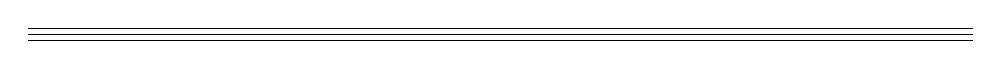
\begin{tikzpicture}\draw (0,0)--(12,0);\draw (0,-0.08)--(12,-0.08);\draw (0,-0.16)--(12,-0.16);\end{tikzpicture}}

\reversemarginpar
\margin{\begingroup\setbox0=\hbox{8}\hbox{\rlap{
\begin{tikzpicture}[overlay,baseline=0pt]\draw[line width=.45pt] (10pt,19pt)--(6pt,22pt)--(-2pt,16pt) .. controls (-10pt,9pt) and (-9pt,-12pt) .. (0pt,-13pt) .. controls (12pt,-12pt) and (18pt,8pt) .. (11pt,17pt);\end{tikzpicture}}\box0}\endgroup{}}
\normalmarginpar

\figure{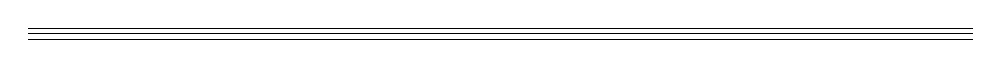
\begin{tikzpicture}\draw (0,0)--(12,0);\draw (0,-0.07)--(12,-0.07);\draw (0,-0.14)--(12,-0.14);\end{tikzpicture}}

\reversemarginpar
\margin{\begingroup\setbox0=\hbox{9}\hbox{\rlap{\begin{tikzpicture}[overlay,baseline=0pt]\draw[line width=.45pt] (3pt,17pt) .. controls (-9pt,21pt) and (-14pt,-10pt) .. (-1pt,-13pt) .. controls (14pt,-13pt) and (23pt,14pt) .. (12pt,19pt) .. controls (8pt,22pt) and (0pt,21pt) .. (3pt,17pt);\end{tikzpicture}}\box0}\endgroup{}}
\normalmarginpar
\uline{p80}\quad 9.2.3\quad $u$ plutôt que $u(q)$

\uline{p82}\quad (9.3.3)\quad $+$ compatibilité avec $R$ ? --

\uline{p87}\quad 9.4.\quad $S$ \uuline{strictement} hensélien ? (on le suppose en p88, $\ell-9$)

pas d'hyp. d'excellence ?

\uline{p91} : 9.5.8.\quad Ne \unsure{mettrait|mettrais}-tu pas une génuflexion ``au signe près''.

\uline{pg92 bis}\quad $S$ est-il strictement hensélien ?

\figure{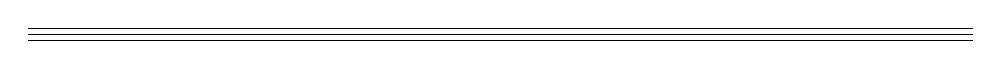
\begin{tikzpicture}\draw (0,0)--(12,0);\draw (0,-0.08)--(12,-0.08);\draw (0,-0.16)--(12,-0.16);\end{tikzpicture}}

\reversemarginpar
\margin{\begingroup\setbox0=\hbox{10}\hbox{\rlap{
\begin{tikzpicture}[overlay,baseline=0pt]\draw[line width=.45pt] (2pt,18pt) .. controls (-14pt,16pt) and (-13pt,-10pt) .. (2pt,-12pt) .. controls (\dimexpr\wd0+16pt\relax,-13pt) and (\dimexpr\wd0+16pt\relax,18pt) .. (\dimexpr\wd0-1pt\relax,20pt) .. controls (5pt,22pt) and (-1pt,17pt) .. (1pt,13pt);\draw[gray,line width=.3pt] (-2pt,14pt).. controls (0pt,20pt) and (4pt,19pt) .. (5pt,17pt);\end{tikzpicture}}\box0}\endgroup{}}
\normalmarginpar
\uline{pg98}\quad 10.5.3.\quad Une extension de $K$ (qui ici est infini) est-elle requise ??.

10.5.4.\quad Dire \uline{où} on fera ces vérifications --

\reversemarginpar
\margin{6}
\normalmarginpar
